\documentclass{scrreprt}

\usepackage{wrapfig}
\usepackage{graphicx}
\usepackage[right=3cm, top=3cm, left=3cm, bottom=3cm]{geometry}
\usepackage[T1]{fontenc}
\usepackage{lmodern}
\usepackage{makeidx}

\makeindex

\author{Carl Levasseur - Pierre Falez - Benjamin Danglot}
\title{Report}

\begin{document}
\maketitle{}

\chapter*{Acknowledgments} %TOREWRITE
\addcontentsline{toc}{chapter}{Acknowledgments}
First, we would like to thank Eddie Gray, our supervisor, who has supported us and
gave us lots of advice throughout this project and the Glasgow Caledonian University for
welcoming us and letting us using their comfortable facilities.\\

Then, we would also like to thank our French supervisor Patrick Lebegue for supporting us
and the University of Lille 1 for giving us the opportunity to carry out our internship in a
foreign country.\\

Finally, we wish to thank all our former professors from the University of Lille 1 who
permits us to achieve our graduation in very good conditions.\\

\chapter*{Abstract}
\addcontentsline{toc}{chapter}{Abstract}
During our 3-month-internship at Glasgow Caledonian University, we had to make a video game.
In this game, every player have a character, called a hero, who has characteristics, spells, ans weapons.
The goals for each player is to be the last survivor.\\

We made it because it touched to several aspects of computer science such as database, network,
programming. Moreover, we had to learn a lot of stuff to get this project done.\\
It was also a good opportunity to work in team, and discover what advantages and disadvantages it comes with.
We used Git to synchronize our works, and we had a lot of issues about it, but it's part of learning.\\

Our project is divided in three parts. First is the client program, which is executed by any people who wants to play,
second is the server, and third is a shared library which contains every network functionnalities that are needed both
by the client and the server.\\

%TOREWRITE
To conclude this abstract we can say that this project was a great experience for many
reasons; we had never worked in team before, we learnt to search and develop
autonomy. Moreover, as it was an Erasmus placement, we could discover a new country,
another language, and last but not least, another culture.

\chapter*{Introduction} %TOREWRITE
\addcontentsline{toc}{chapter}{Introduction}
In order to validate our DUT diploma, we chose to carry out our internship in an
English speaking country to improve our English language.\\

Our supervisor, Richard Foley, offered us a project's subject based on web and mobile
technologies. We accepted it because we thought it was a really good idea to work on future
technologies and it permits us to explore several fields using our computer skills acquired
during our studies.\\

The project aimed to achieve a usable system by professors and able to manage
multiple choice questions in an amphitheatre. Two mobile applications also had to be
created so that students can answer the quiz.\\

This report consists of three parts. We will first realise an overall presentation of the
project and its objectives. We will then, in a second part, describe how the system can
handle the quizzes and how the corresponding mobile applications work. Finally, we will
review this project and the skills acquired during these three months.

\renewcommand{\contentsname}{Summary}
\tableofcontents

\part{Project presentation}
\chapter{Workplace}
\section{Glasgow}%TOREWRITE
Glasgow is the largest city in Scotland and third most populous in the United
Kingdom. The city is situated on the River Clyde in the country's West Central Lowlands.
Today it is one of Europe's top ten financial centres and is home to many of
Scotland's leading businesses. Glasgow is also ranked as the 57th most liveable city in the
world.\\

In the late 19th and early 20th centuries Glasgow grew in population, eventually
reaching a peak of about 1 million in 1939, and was the fourth-largest city in Europe, after
London, Paris and Berlin. In the 1960s, comprehensive urban renewal projects resulting in
large-scale relocation of people to new towns and peripheral suburbs, followed by
successive boundary changes, have reduced the current population of the City of Glasgow
council area to 600,000, with 1,200,000 people living in the Greater Glasgow urban area. The
entire region surrounding the conurbation covers approximately 2.3 million people, 41\% of
Scotland's population.\\

The heart of the city is George Square, located in the city centre, site of many of
Glasgow's public statues and the elaborate Victorian Glasgow City Chambers, headquarters
of Glasgow City Council.\\

Three Universities are present in Glasgow: University of Glasgow, University of
Strathclyde and Glasgow Caledonian University. We achieved our project in this latter.

\section{Glasgow Caledonian University}%TOREWRITE
Glasgow Caledonian University is a public University. The university was constituted
by an Act of Parliament on 1 April 1993 as a result of a merger between Glasgow Polytechnic
and The Queen's College. It has 17,500 students from over 100 countries, almost 400
different courses available, a modern city-centre campus in Glasgow and high-tech facilities,
including the award-winning Saltire Centre library.

\section{Workspace}
The project was mainly realised in our flats because we already had everything we needed there:
computers, high-speed Internet connection and softwares. Moreover, we prefered to use our laptops
instead of university's computers because our tools were already configured.

\section{Project definition}
\subsection{Project description} %TODO Update for each functionnality implemented
The project consists in creating a video game where each player has its own character, also 
called a hero. A hero has several characteristics such as % Caracteristiques ici
spells, and can level up by beating his enemy. The goal is to be the last survivor.

\part{How to play}
\section{Login screen}
\section{Managing your characters}
\subsection{Creating a new character}
\subsection{Statistics}
\subsection{Skill-tree}
\subsection{...}
\section{Launch a new game}
\section{Join an existing game}
\section{In-game}
\subsection{In-game screen}
\subsection{Movement}
\subsection{Attack}
\subsubsection{Auto-attack}
\subsubsection{Skills}
\subsection{Camera}
\subsection{How to win ?}
\section{End-game}

\part{Technical description}
\chapter{Technical choices}
\section{Programming language}
We used C++ all along this project, because it provides interesting libraries for making video games, such as SFML.
Moreover, JAVA is the only oriented-language we studied at the university, so it enabled us to become multi-skilled.
Finally, we wanted to try the boost libraries, which allow programmers to make robust C++ programs much more easily, and improve
software portability.

\section{External libraries}
\subsection{Boost} %TODO
\begin{center}

\includegraphics[scale=0.75]{Boost.png}
\end{center}
Boost is a set of libraries for the C++ programming language that provide support for tasks and structures such as linear algebra, pseudorandom number generation, multithreading, image processing, regular expressions, and unit testing. Release 1.52 contains over eighty individual libraries.\\

Most of the Boost libraries are licensed under the Boost Software License, designed to allow Boost to be used with both free and proprietary software projects. Many of Boost's founders are on the C++ standards committee, and several Boost libraries have been accepted for incorporation into both Technical Report 1 and the C++11 standard.

\subsection{SFML} %TODO
\label{SFML}

\begin{center}

\includegraphics[scale=0.75]{SFML2.png}
\end{center}

SFML (Simple and Fast Multimedia Library) is a portable and easy-to-use API for multimedia programming. It is written in C++ but bindings are available for C, D, Python, Ruby, OCaml, .Net. It is an object oriented alternative for the SDL.\\

SFML provides 2D graphics that are hardware accelerated with OpenGL. SFML can also be used for OpenGL windowing. SFML also provides different modules made to ease programming games and multimedia applications. SFML site offers complete SDK bundle in single pack, and tutorials to ease the developers. SFML Source code is provided under the terms of the zlib/png license.

\subsection{MySQL}
MySQL is the world's most widely used open source relational database management system that runs as a server providing multi-user access to a number of databases.

\chapter{How it work}
\section{Graphics}
\subsection{Modeling maps}
Maps are handled by a two-dimension-array which contains Case objects. Each Case object contains attributes \emph{x} and \emph{y} to describe its coordinates. Another attribute allow us to know if a character can cross it. Finally, there is an attribute which contains a texture-id so that we know how to display it. In order to get these maps persistent, we wrote it in binary files. At the beginning, we had to do it manually, but it was tedious to do, so we developped a simple program to make it easier.\\

Both for performances and ergonomic, we decided to make a map editor, with a texture-palette. Thus, we can create new maps just by using the mouse, with two layers to handle the element overlay, then we can save it and load it into the game. The game display the map by reading its binary file, once it knows the id of each Case, it paint the corresponding texture at Case's coordinates.

\begin{figure}
\begin{center}
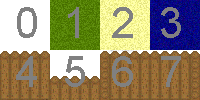
\includegraphics{image1.png}
\end{center}
\caption{Textures list}
\end{figure}

\subsection{Modeling characters}
Modélisation du personnage:
Le personnage est déssiné dans 3 positions différentes (immobile, pas gauche, pas droit)pour les 4 directions possibles (SUD, EST, OUEST, NORD). Chaque direction est modélisée par un attribut int dans la classe personnage.

Every characters are drawn in three different positions: still, ... Each direction is represented by an attribute in Personnage's class.
\subsection{Camera}
The Camera object permit to display a part of map, depending on its position and its range\footnote{the window size}. Thus, the program only draw visible part of the map. We can move the camera either with the directionnal arrows or by moving the mouse on window edges. The movement is done pixel by pixel instead of case by case in order to be more fluid.

\section{Network}
\subsection{libnetwork}
\subsection{Client}
\subsection{Server}

\section{Gameplay}
\subsection{Server}
\subsubsection{Game rules}
Mode de jeu :
Les modes de jeu sont implémentés grâce à une classe abstraite qui régis toutes les règles de jeu : spawn des équipes, règle de jeu : temps, type de score (kill, capture de drapeau), carte a utiliser etc...



\end{document}
